\section{Introduction}
\label{sec:introduction}

\subsection{Product Description}

\begin{figure}[H]
    \centering
    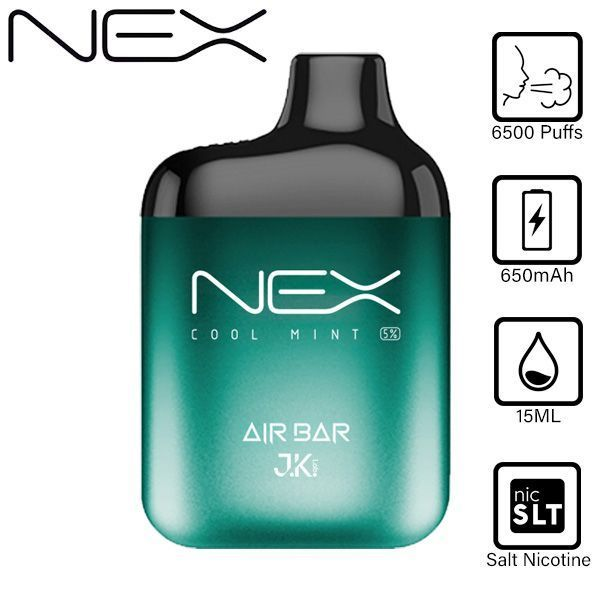
\includegraphics[width=0.5\linewidth]{airbar.jpg}
    \caption{NEX Vape Air Bar: Current Design}
    \label{fig:product_photo}
\end{figure}

\begin{figure}[H]
    \centering
    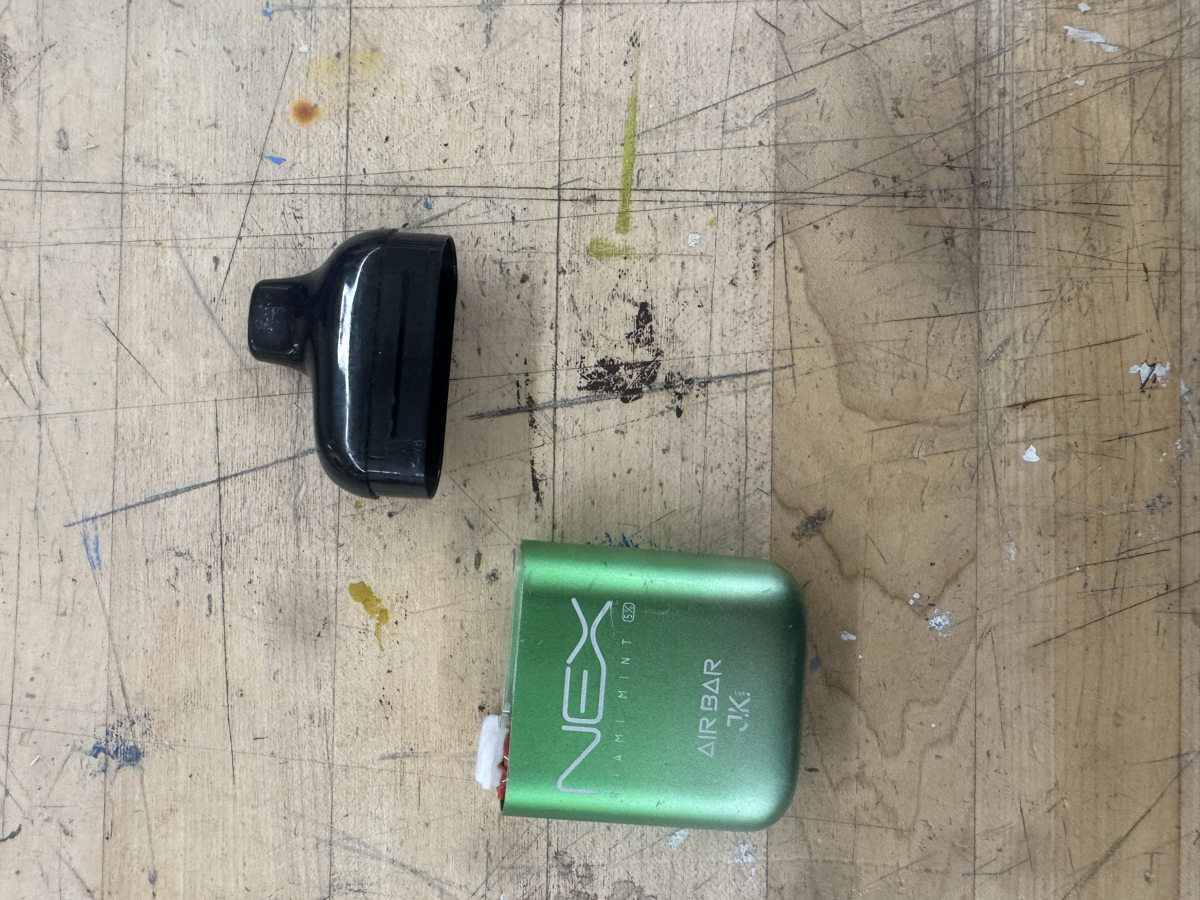
\includegraphics[width=0.5\textwidth]{figures/makerspace/IMG_6130.png}
    \caption{The Air Bar NEX 3K disposable e-cigarette with mouthpiece separated from the aluminum housing.}
    \label{fig:product_disassembled}
\end{figure}

The product selected for this project is a disposable electronic cigarette (e-cigarette), also known as a single-use vape. The NEX Vape Air Bar is a new model of e-cigarette. It can be purchased at most smoke shops for a price of 8 to 15 dollars.

A disposable e-cigarette is a self-contained, battery-powered device that heats a liquid solution (``e-liquid'') containing nicotine, propylene glycol, vegetable glycerin, and flavorings to produce an inhalable aerosol. The device is designed for single use: once the e-liquid is depleted or the battery is exhausted (typically after 200--800 puffs), the entire unit is discarded.

\subsection{Functionality Analysis}

The operating principle is straightforward: when the user inhales, an airflow sensor on the printed circuit board (PCB) detects the pressure change and activates the battery circuit. The lithium-ion battery then delivers current to a resistive heating coil (the atomizer), which rapidly heats to approximately 200--300\,$^{\circ}$C. The coil is wrapped around an absorbent cotton wick saturated with e-liquid. The heat vaporizes the liquid, producing an aerosol that the user inhales through the mouthpiece.

Key functional subsystems:
\begin{enumerate}
    \item \textbf{Power supply}: Lithium-ion or lithium-polymer cell (typically 280--1000\,mAh, 3.7\,V nominal)
    \item \textbf{Control electronics}: PCB with airflow sensor, battery protection IC, and LED indicator
    \item \textbf{Atomization}: Resistive coil (kanthal or nichrome wire) wound around cotton wick
    \item \textbf{Fluid storage}: Absorbent reservoir holding 2--15\,mL of e-liquid
    \item \textbf{Enclosure}: Outer housing (aluminum or plastic) with integrated mouthpiece
\end{enumerate}

\subsection{Scope of Analysis}

This project analyzes the \textbf{entire product} rather than a subassembly. The device consists of 8 distinct parts, satisfying the project requirement of at least five parts. Among these parts, we identify at least three different material types including two metallic materials (Section~\ref{sec:materials}), and at least three parts requiring multiple manufacturing processes (Section~\ref{sec:processes}).

\subsection{Designed Usage and Durability}

Disposable e-cigarettes are engineered for a single-use lifecycle. The designed usage is approximately 6500 puffs, after which the device is intended to be discarded. There is no designed mechanism for recharging, refilling, or servicing. The battery, which Oxford and UCL researchers demonstrated is capable of over 450 charge--discharge cycles \cite{williams2023}, is used exactly once before disposal.

\subsection{Motivation: The E-Waste Crisis}

The environmental impact of disposable e-cigarettes is substantial and growing:
\begin{itemize}
    \item Over 840 million vaping devices are discarded globally each year, at a rate of approximately 5.7 devices per second \cite{pirg2024}.
    \item An estimated 30 tons of lithium from e-cigarette batteries enters landfills annually---enough to produce approximately 3,350 electric vehicle batteries \cite{recyclenation2025}.
    \item Improperly discarded lithium-ion batteries cause waste facility fires costing at least \$95 million per year in the United States \cite{wmw2025}.
    \item A 2024 study found that 52.9\% of U.S. e-cigarette users aged 15--24 dispose of devices in regular trash \cite{truth2024}.
\end{itemize}

This project investigates how Design for Disassembly (DfD) principles can be applied to redesign the disposable e-cigarette, with the central goal of enabling efficient battery recovery and recycling through a proposed universal removable battery standard.
